% article example for classicthesis.sty
\documentclass[10pt,a4paper]{article} % KOMA-Script article scrartcl
\usepackage{lipsum}
\usepackage{url}
\usepackage[nochapters]{../classicthesis} % nochapters
\usepackage{graphicx}
\graphicspath{ {img/} }
\usepackage{booktabs}
\usepackage{float}
\usepackage{subfloat}
\usepackage{subfig}
\usepackage{hyperref}
\usepackage[ngerman]{babel}



\begin{document}
    \pagestyle{plain}
    \title{\rmfamily\normalfont\spacedallcaps{Mission: Chuckhole}}
    \author{\spacedlowsmallcaps{Marwan ElMezni, Michael Moosbauer}}
    \date{} % no date
    
    \maketitle
    
% picture titles still german

    \tableofcontents
    


    \section{Motivation and problem statement}

	

Even though municipalities try to maintain and repair roads, many segments still contain chuckholes that vehicle owners prefer to avoid to drive or to bike on because they would so likely damage their vehicles and slow or interrupt the traffic.\\
This was the background motivation to develop a mobile application, in a biking context, that helps users to avoid damaged sections of roads or to detect and localize chuckholes.

    \section{Recommended Setup}

	In order to use the main app \textbf{Mission:Chuckhole}, some requirements are needed.\\
	Of course, you need a bike to drive along the streets.
	For the test rides, two bikes have been used:

	\begin{itemize}
		\item \textbf{Dr"ossiger XRA 650 B}: full suspension All-Mountain-bike (150mm/155mm suspension)
		\item \textbf{Rotwild G1 2016}: full suspension Downhill-bike (203mm/203mm suspension)
	\end{itemize}
	%bike pictures
	In order to fix the smartphone on the bike, it is recommended to buy a smartphone fix to safely fix your phone on the handlebar. One good possibility is the mumbi TwoSave smartphone fix depicted in \autoref{fig:smartphone_fix}:
	
	\begin{figure}[H]
		\begin{center}
 		  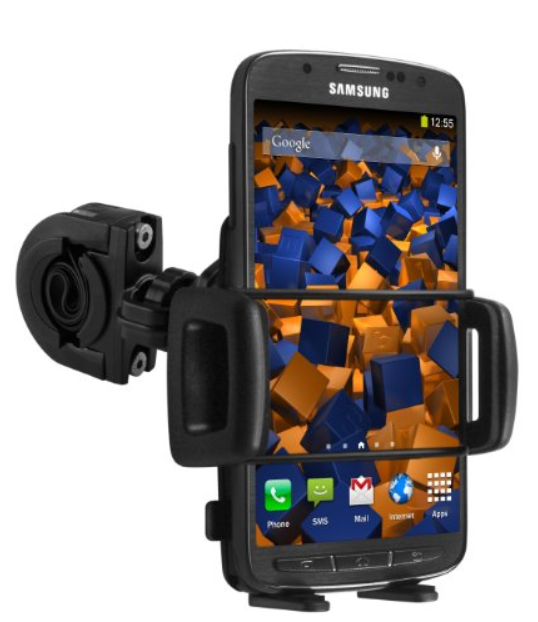
\includegraphics[scale=0.3]{smartphone_fix}
		  \caption{mumbi TwoSave smartphone fix}
		  \label{fig:smartphone_fix}
		\end{center}
	\end{figure}
	\noindent
	It is suitable for many modern smartphones and provides a good multiple-fixing system so your phone is well protected.\\
	Last requirement is of course that our \textbf{Mission:Chuckhole} app is installed on the used phone.
	During development, we used mostly two different devices: a Samsung Galaxy S4 Active and a Google Nexus 5X.
	On both devices, the app ran smoothly and without any problems.


    \section{Basic Implementation idea}
	
	In order to determine the quality of roads, we will use the g force physical notion. 
	It represents the force that acts on every object that is moved somehow. 
	In context of \textbf{Mission:Chuckhole}, the forces are measured that act on the smartphone.
	From these values, it is possible to detect great changes, which can be interpreted as chuckholes.
	Android phones are equipped with an acceleration sensor that provides values for the forces acting in x, y and z direction.
	Each g force value calculated of these three single values will be associated with a corresponding location provided by GPS.
	The data will be stored locally into an SQLite database to access them again in future app launches.\\
	\autoref{fig:arch_flow} gives an overview of the main parts of \textbf{Mission:Chuckhole}:
	
	\begin{figure}[H]
	\centering
    	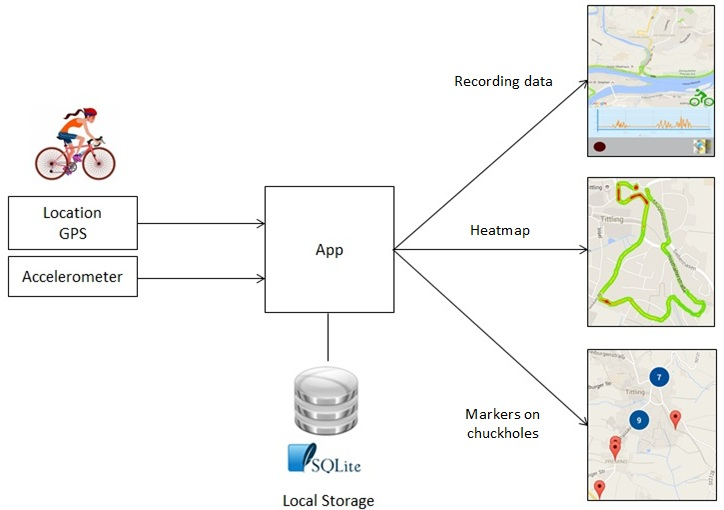
\includegraphics[scale = 0.8]{pic1}
    	\caption{Architecture and flow of information of the app }
	\label{fig:arch_flow}
    	\end{figure}
    
	\noindent
	The next section describes these app features more detailed.
    
    \section{App components and features}
	% pictures etc. here
    
    
    \textbf{Onboarding}\\
    New users will start with an initiation to get an overview about the mode of operation and main functionalities of the app. In subsequent uses, this phase will be skipped.\\
    %explain figure: every single figure, what it shows, ... - in full sentences!
    First, the onboarding screen will show the user how to start the recording phase. He has to press the green bike picture everytime he wants to move to the next initiation step. \\
    Second, the attention of the user will be directed to the live visualization graph of g-force values that will be displayed during the ride.\\
    Third, the user will be informed that he can check results of his recording session using the 'heatmaps and markers overlay' features.
    

	\begin{figure}[H]
	  \centering
	  \subfloat[Onboarding site 1]{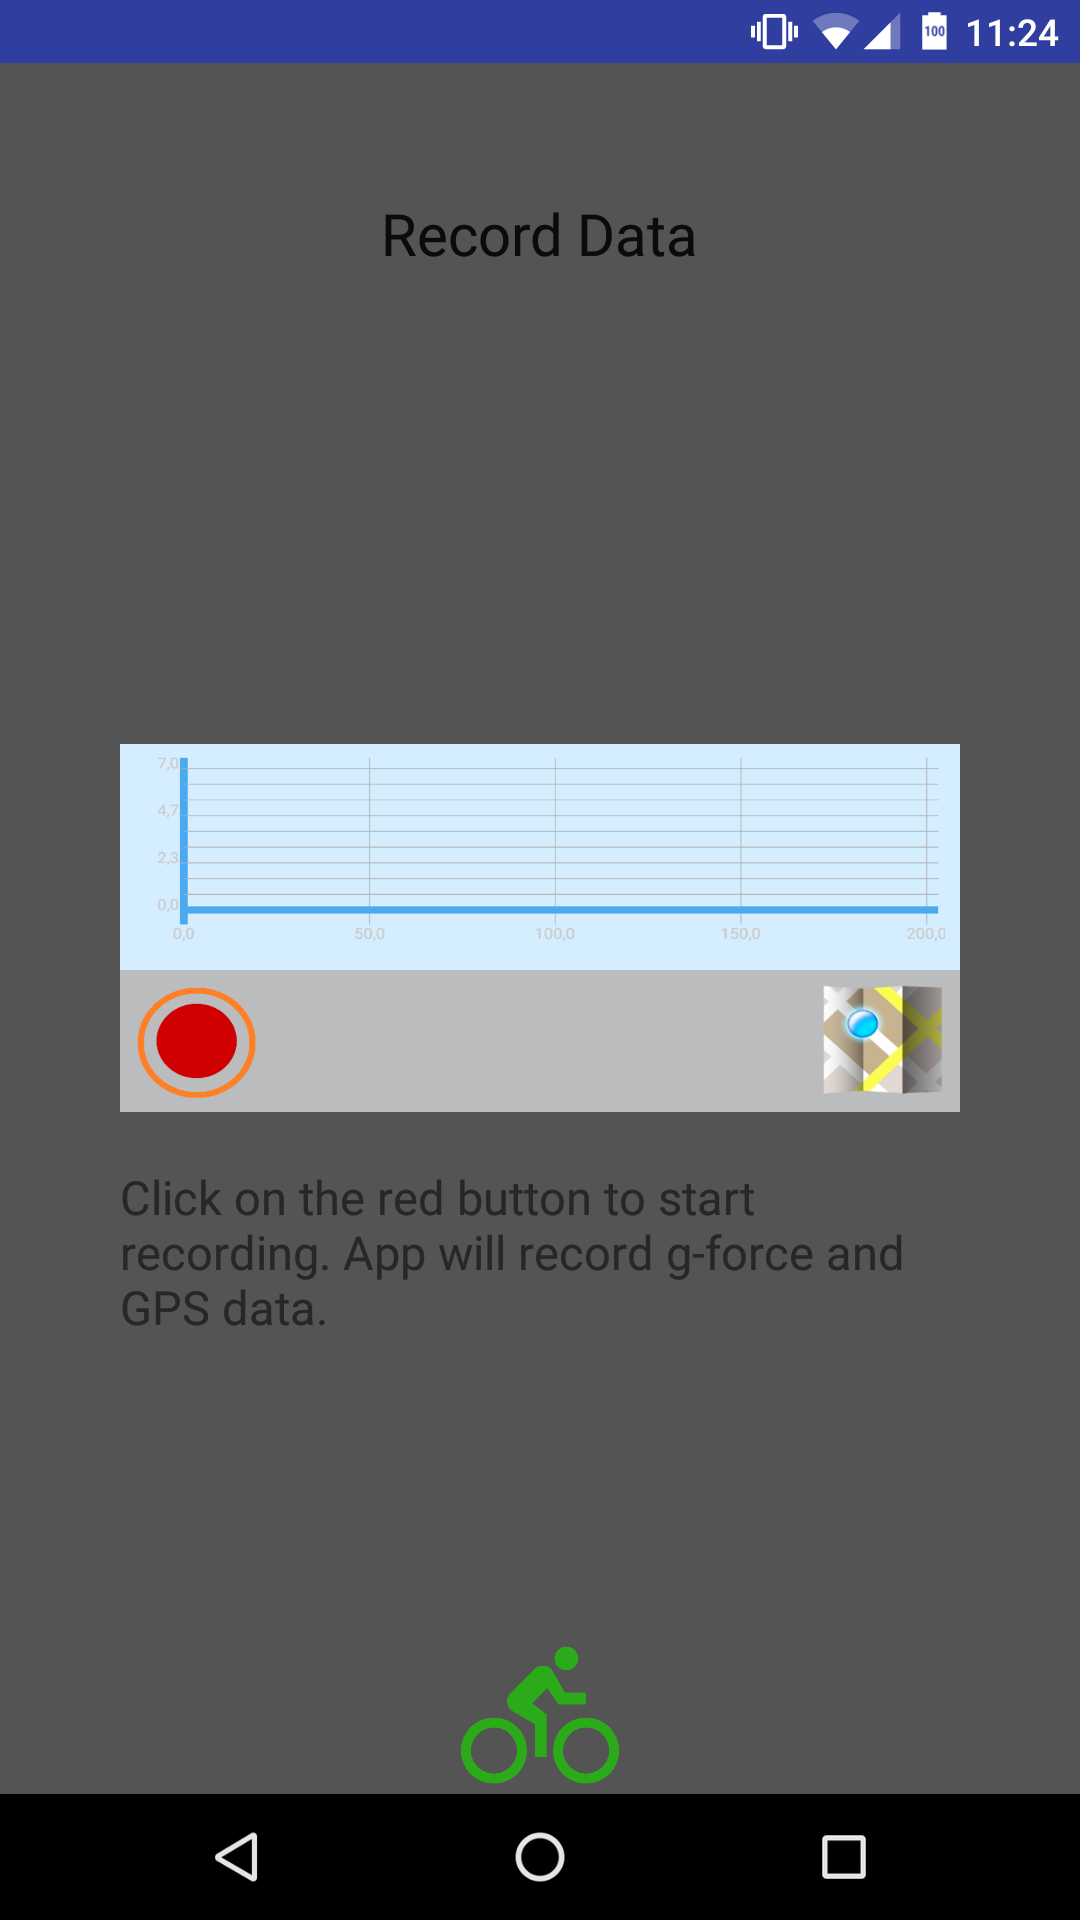
\includegraphics[width=0.25\textwidth]{pic7}\label{fig:onboarding_1}}
	  \hfill
	  \subfloat[Onboarding site 2]{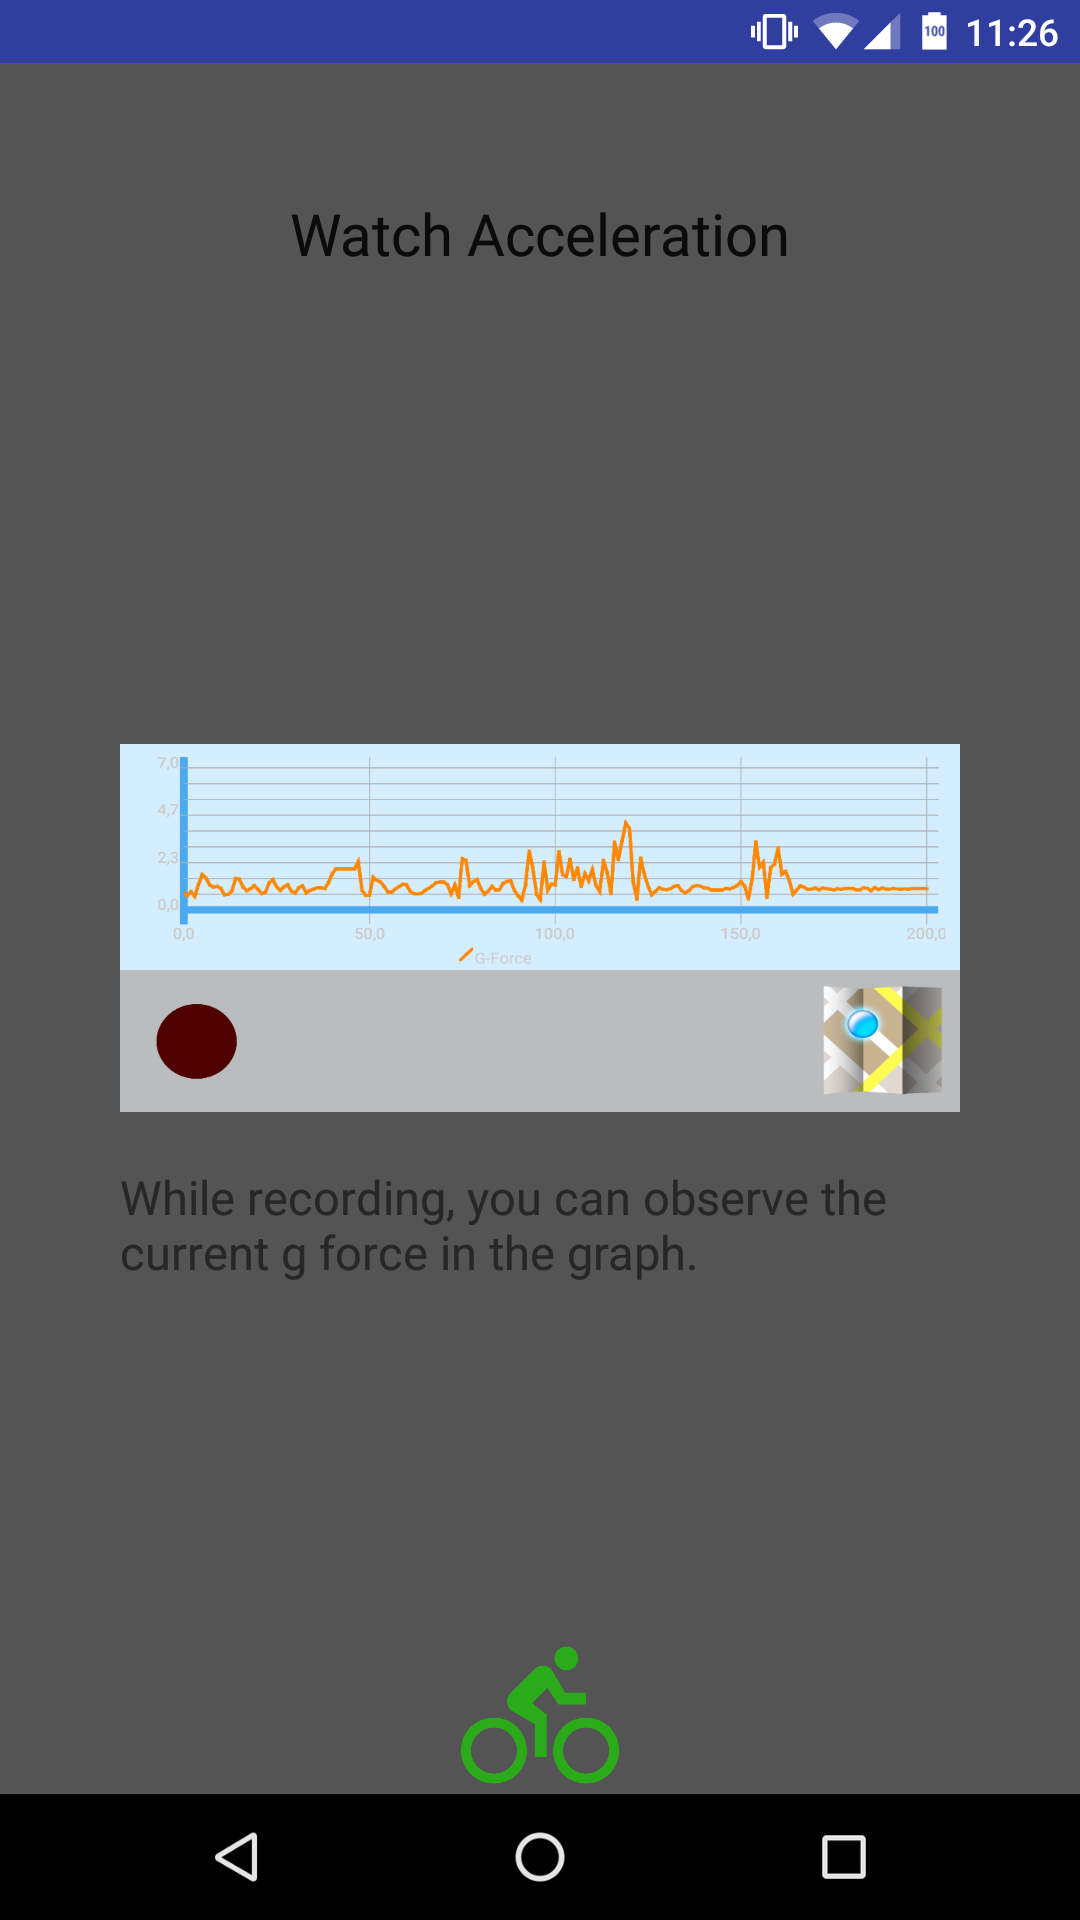
\includegraphics[width=0.25\textwidth]{pic8}\label{fig:onboarding_2}}
	  \hfill
	  \subfloat[Onboarding site 3]{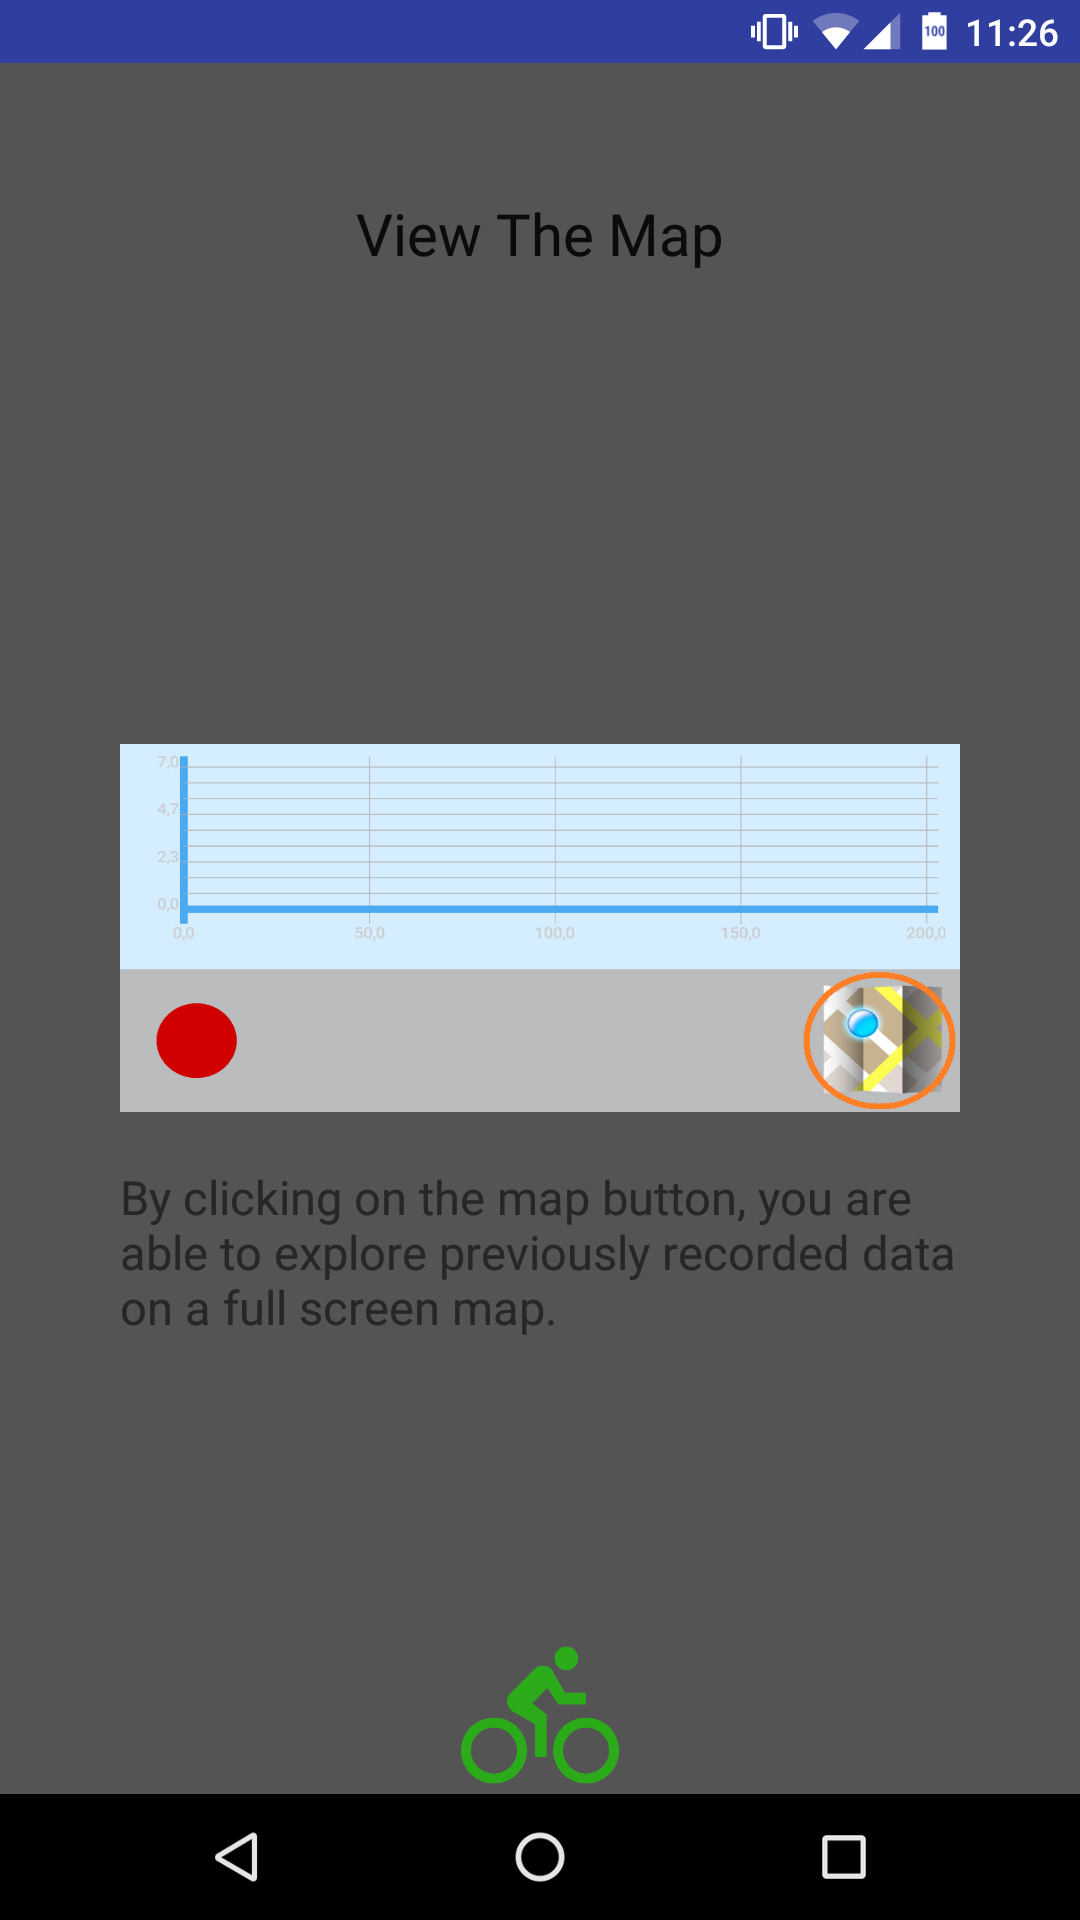
\includegraphics[width=0.25\textwidth]{pic9}\label{fig:onboarding_3}}
	  \caption{Onboarding at first App start}
	  \label{fig:onboarding}
	\end{figure}
	
	\noindent
	\textbf{Google Map}\\
    Some features require a google map. It was added to the app using the Google Maps Android API which automatically handles access to Google Maps servers, data downloading, map display, and response to map gestures. 
    We also used API calls to add heatmap and markers overlay in clusters.

    \subsection{ Recording data}
    	This feature allows an app user to check the quality of roads during a bike ride.
    	Using the accelerometer sensor, the app will get the three acceleration axes' values (x, y and z) that are necessary to calculate the g-force by applying the following formula:

    
	\begin{center}
		$ gforce = \frac{\sqrt{x^2 + y^2 + z^2}}{gforce\_earth} $
	\end{center}
	\noindent
    \textbf{Input}\\
    A user has to press the recording button to start the recording phase and once again to stop it.
    For a better visual distinction at the user side, the button has two different colors depending on its status: brown when it is pressed and red otherwise.\\
    A user may also want to use the 'Heatmap overlay'  or 'markers on chuckholes' features at once or simultaneously and this is possible by pressing the button on the right bottom.\\
    \textbf{Ouput}\\
    The green bike picture is a sign that the ride has just started.\\
    The graph shows the change of the g-force value during the ride and serves as a second output feedback to assure the user that recording is working well.\\
    Both will appear after pressing the recording button.\\
    The third output element is the heatmap that shows the heatmap overlay of previous recording sessions. Moreover, it's dynamically updated to provide real time overlay of the current session.
    
    \begin{figure}[H]
	\centering
    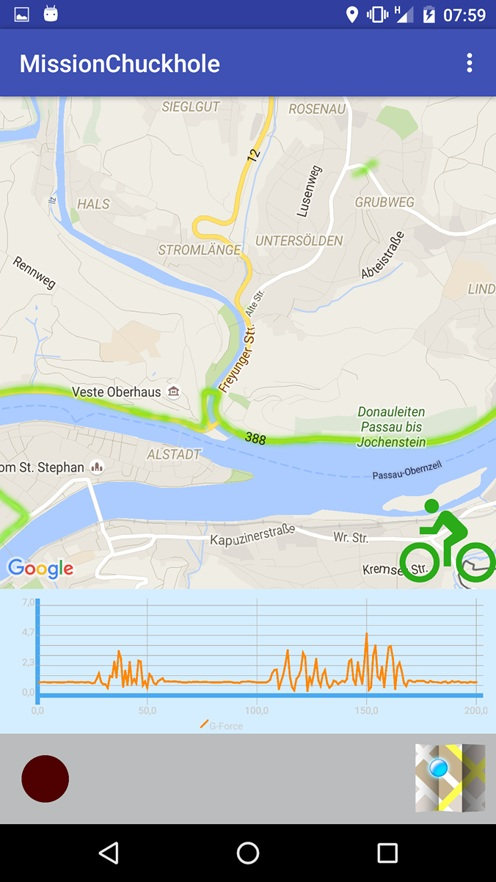
\includegraphics[scale=0.4]{pic2}
    \caption{Recording data during a bike ride }
		  \label{fig:record_data}
    \end{figure}
    \noindent
    \textbf{Storage}\\
    Local storage was done via an SQLite database because ...\\
    DataStore is an intermediate data structure between the app features and the SQLite database. Each record of the Datastore contains the following attributes: ...
    
    
    \subsection{ Heatmap Overlay}
    
    Heatmaps make it easy for viewers to understand the distribution and relative intensity of data points on a google map and was overlaid using the Google Maps Android Heatmap Utility.\\
    We opted for a dynamic heatmapping that requires a collection of 'weighted' latitude/longitude coordinates, each with an intensity value that will determine its associated color.
    Highest values of intensity will be mapped by default to red while lowest ones to green. Concerning the values in between, the given color is generated using interpolation between red and green. \\
    Our collection will retrieve locations from the DataStore structure and their corresponding g-force values which will represent the intensity parameter. Consequently, locations on a smooth road will get green color while chuckholes will be colored in red and points with average g-forces values will be in yellow.\\
    So an app user will be able to avoid damaged sections of roads or view areas that haven't been checked yet.
     
    \begin{figure}[H]
    \centering
	   
       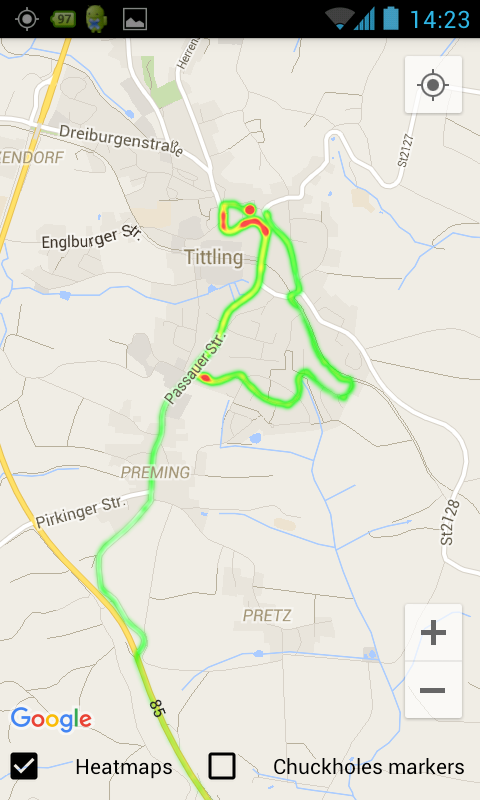
\includegraphics[scale = 0.31]{pic4}
       \caption{Overlay of heatmap after a bike ride}
		  \label{fig:heatmap_overlay}
       
    \end{figure}
    
    
    
    
    
    \subsection{ Markers on chuckholes Overlay}
    
    This feature is the second output option for an app user who may want to view locations of chuckholes that were detected during a bike ride in a simple way. The locations are retrieved from the DataStore structure described previously. Using the Google Maps Android Marker Clustering Utility, a marker will be overlaid on each location where the corresponding g-force level reaches or exceeds a specific threshold value = 3.5. \\
    When a user views the map at a high zoom level, individual markers will be shown on the map. When a user zooms out, the markers gather together into clusters, to make viewing the map easier.
    
    \begin{figure}[H]
    \centering
	
	   
       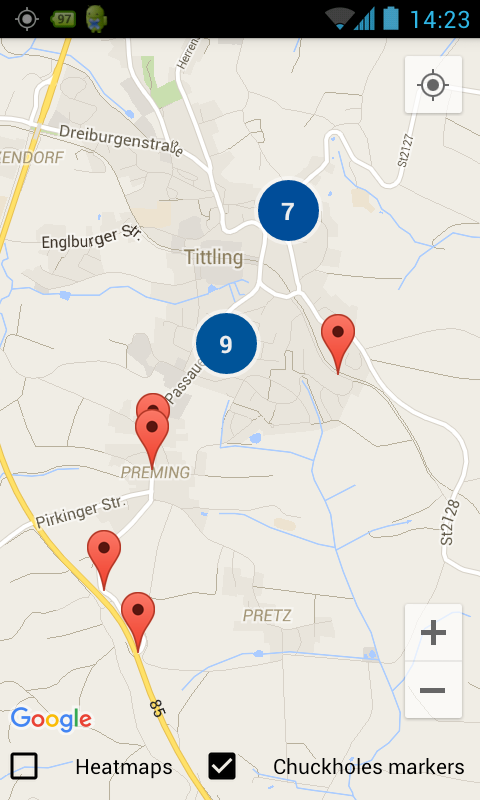
\includegraphics[scale=0.31]{pic3}
    \caption{Markers on chuckholes in clusters}
		  \label{fig:markers_overlay}
       
        \end{figure}
    
    

    
    

    \section{Problems faced during implementation and lessons learned}
\subsection{Problems}


Unfortunately, the heatmap utility suffers from some limitations [1]. The main handicap that affects our overlay is that the heatmaps circles overlap at low zoom levels which causes fake coloring and this is due to the fact that the 'Intensity' parameter is additive: the overlap area of two circles of intensity 1 will lead to an overall intensity 2.
    
    \begin{figure}[H]
    \centering
	   
       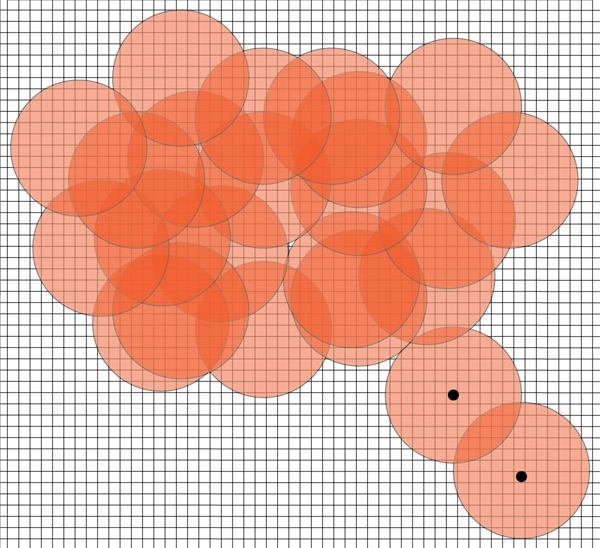
\includegraphics[scale =0.4]{pic6}
    \caption{Overlaps of heatmaps' circles at low zoom levels}
		  \label{fig:overlaps}
       
    \end{figure}
    \noindent
    To overcome this issue, we apply a filtering on our dataset, within a specific zoom range where the overlaps occur, in an attempt to reduce fake coloring of heatmaps.

\subsection{Lessons}

This project was a good occasion to check out the Google maps API for android. However, it suffers from few limitations so it is necessary to review regularly the releases’ notes and updates.

    
    
    
    % bib stuff
    \nocite{*}
    \addtocontents{toc}{\protect\vspace{\beforebibskip}}
    \addcontentsline{toc}{section}{\refname}    
    \bibliographystyle{plain}
    
    \bibliography{Bibliography}

    
    
    
    
\end{document}
